\documentclass{standalone}

\usepackage{tikz}

\begin{document}
	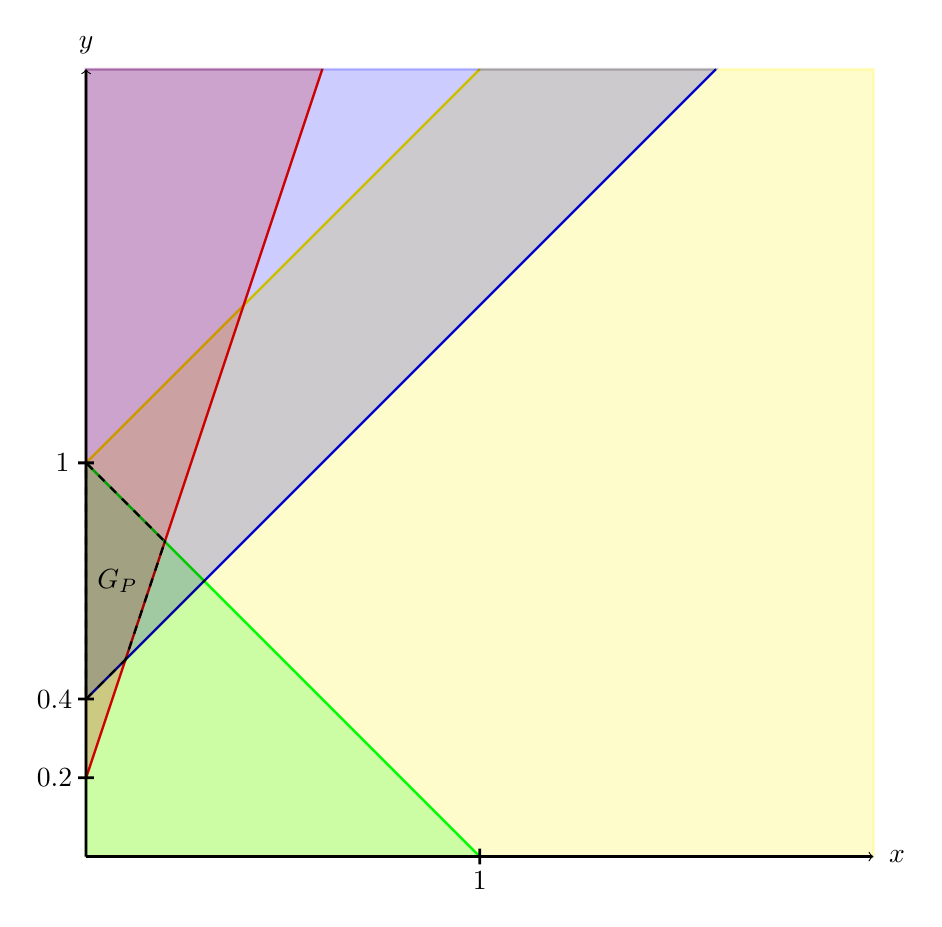
\begin{tikzpicture}{scale=0.5}
		\begin{scope}[transparency group]
		\begin{scope}[blend mode=multiply]
		\draw[->] (0,0) -- (10,0);
		\draw[->] (0,0) -- (0,10);
		\node at (10.3,0) (y) {$x$};
		\node at (0,10.3) (x) {$y$};
		
		\draw (-0.1,5) -- (0.1,5);
		\node at (-0.3,5) (1y) {1};
		\draw (-0.1,2) -- (0.1,2);
		\node at (-0.4,2) (0.4y) {0.4};
		\draw (-0.1,1) -- (0.1,1);
		\node at (-0.4,1) (0.4y) {0.2};
		\draw (5,-0.1) -- (5,0.1);
		\node at (5,-0.3) (1x) {1};
		
		\draw[yellow,thick] (0,5) -- (5,10);
		\draw[green,thick] (0,5) -- (5,0);
		\draw[blue,thick] (0,2) -- (8,10);
		\draw[red,thick] (0,1) -- (3,10);
		
		\draw[yellow, fill=yellow, opacity=0.2] (0,5) -- (5,10) -- (10,10) -- (10,0) -- (0,0) -- (0,5);
		\draw[green, fill=green, opacity=0.2] (0,5) -- (5,0) -- (0,0) -- (0,5);
		\draw[blue, fill=blue, opacity=0.2] (0,2) -- (8,10) -- (0,10) --(0,2);
		\draw[red, fill=red, opacity=0.2] (0,1) -- (3,10) -- (0,10) -- (0,1);
		
		\draw[dashed, thick, black] (0,2) -- (0.5,2.5) -- (1,4) -- (0,5) -- (0,2);
		\node at (0.4,3.5) (GP) {$G_P$};
		\end{scope}
		\end{scope}
	\end{tikzpicture}\\
	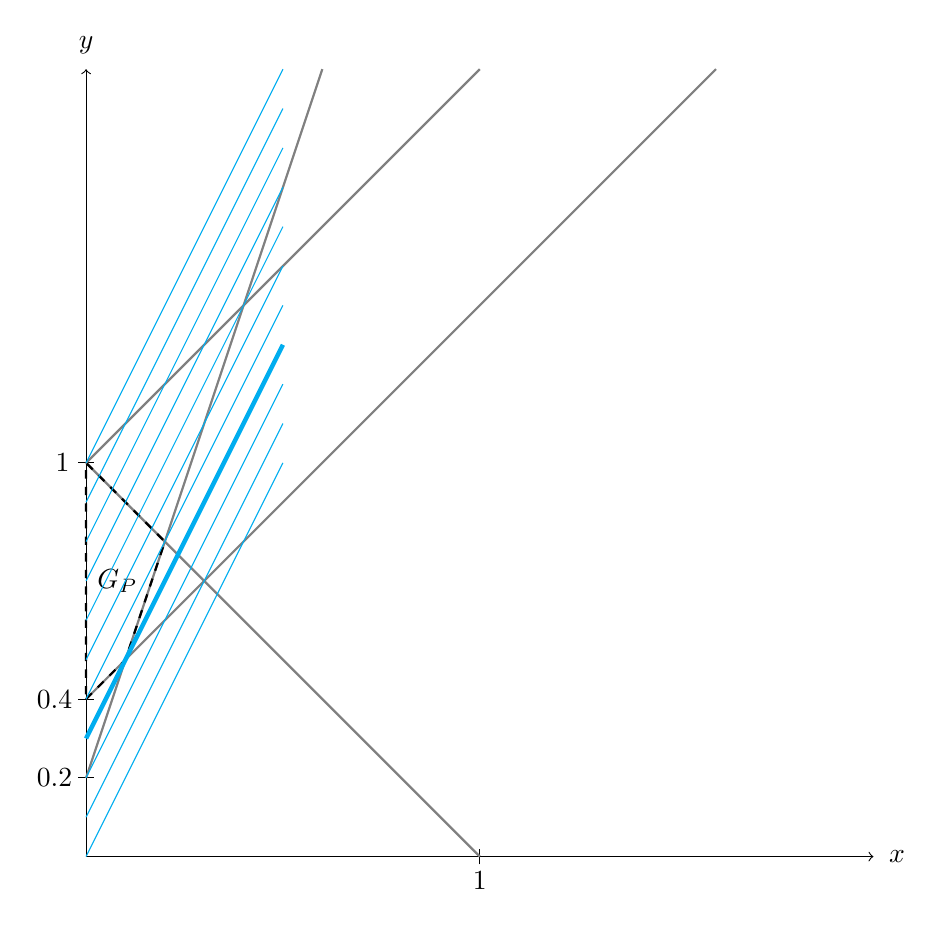
\begin{tikzpicture}
		\draw[->] (0,0) -- (10,0);
		\draw[->] (0,0) -- (0,10);
		\node at (10.3,0) (y) {$x$};
		\node at (0,10.3) (x) {$y$};
		
		\draw (-0.1,5) -- (0.1,5);
		\node at (-0.3,5) (1y) {1};
		\draw (-0.1,2) -- (0.1,2);
		\node at (-0.4,2) (0.4y) {0.4};
		\draw (-0.1,1) -- (0.1,1);
		\node at (-0.4,1) (0.4y) {0.2};
		\draw (5,-0.1) -- (5,0.1);
		\node at (5,-0.3) (1x) {1};
		
		\draw[gray,thick] (0,5) -- (5,10);
		\draw[gray,thick] (0,5) -- (5,0);
		\draw[gray,thick] (0,2) -- (8,10);
		\draw[gray,thick] (0,1) -- (3,10);
		
		\draw[dashed, thick, black] (0,2) -- (0.5,2.5) -- (1,4) -- (0,5) -- (0,2);
		\node at (0.4,3.5) (GP) {$G_P$};
		
		\draw[cyan] (0,5) -- (2.5,10);
		\draw[cyan] (0,4.5) -- (2.5,9.5);
		\draw[cyan] (0,4) -- (2.5,9);
		\draw[cyan] (0,3.5) -- (2.5,8.5);
		\draw[cyan] (0,3) -- (2.5,8);
		\draw[cyan] (0,2.5) -- (2.5,7.5);
		\draw[cyan] (0,2) -- (2.5,7);
		\draw[cyan, ultra thick] (0,1.5) -- (2.5,6.5);
		\draw[cyan] (0,1) -- (2.5,6);
		\draw[cyan] (0,0.5) -- (2.5,5.5);
		\draw[cyan] (0,0) -- (2.5,5);
	\end{tikzpicture}
\end{document}